
\chapter{Requirements for MPTCP Reassembly} \label{chap:reassembly}

Now that we've gone over how Bro performs reassembly for regular TCP traffic, we must now adapt the mechanism to process MPTCP traffic. This section will describe which components are needed in order to achieve this objective. As we will see, these changes can be brought about in a variety of ways, and can be performed at various stages of the Engine's operation. Going forward, we will use the following assumptions:
\begin{itemize}
\item MPTCP traffic that we attempt to reassemble behaves correctly. If ever the protocol is misused, we will rely on scripts such as those developed in the first iteration to deal with it.
\item Identifying MPTCP connections by the tokens is sufficient. As we've mentioned before, the tokens are not meant to be globally unique and may collide with traffic from multiple hosts. We will, however, consider them sufficient for the time being.
\end{itemize}

As a reminder, we saw in chapter \ref{chap:recap} that all modifications must be made within the Engine to ensure the reassembled data can be processed by the full analyzer tree.

\section{Maintaining an MPTCP Connection List}
In order to reassemble data from multiple TCP subflows into a single MPTCP flow, it is first necessary to ensure that Bro is able to recognize which flows belong together. In order to do this, we will have to recompute the mappings from all the hosts whose traffic we see. This process is similar to what we used in the connection logging script of chapter \ref{chap:script}. However, since the Engine grants us easy access to cryptographic libraries such as OpenSSL \cite{openssl} which is already used for md5 hashing (and basing ourselves on the second assumption), we will perform the matching based on the tokens rather than on the address advertisement.\\

Similarly to what is done for transport layer protocols, we will maintain a dictionary of all the ongoing MPTCP Connections. In addition, we will maintain a second dictionary mapping subflows to their MPTCP connections. The following pseudo-code illustrates how one could populate such dictionaries:

\begin{code}
if (MP_Capable & SYN+ACK) {
	token1 = mp_token_hash(key1)
	token2 = mp_token_hash(key2)
	mp_conns.Insert(token1, this_connection)
	mp_conns.Insert(token2, this_connection)
	mp_flows.Insert(this_connection, this_connection)
}

if (MP_Join & SYN) {
	connection = mp_conns.Lookup(token)
	mp_flows.Insert(this_connection, connection)
}
\end{code}

As we can see, we need to be able to identify which MPTCP connection a subflow is joining; this is made possible by \texttt{mp\_conns}. The tokens that are found at the connection initiation are used as keys, so that joins can then perform a simple lookup to find the initial connection. Of course, if no result is found during the lookup, then the original connection was not observed and we are limited at attempting partial reassembly or defaulting to standard TCP processing. On the other hand, if the key is already present at the MP\_Capable stage, then there is a token collision. If the first connection using this token has been terminated, then Bro's Engine provides us with mechanisms for clearing the dictionary entry. The other case (two different hosts trying to use the same token) is not considered given assumption two. The second dictionary, \texttt{mp\_flows} is used to match the identifying 5-tuple of the TCP connection to the original MPTCP subflow. This will be necessary down the road, since subsequent packets will not carry the token. \\

Operations on the other stages of the TCP handshakes (both for MP\_Capable and MP\_Join) are not necessary. For MP\_Capable, all we need are the two keys and 5-tuple which are all present in a single header at the SYN+ACK stage, and this allows us to avoid token computations if the use of MPTCP is refused at an early stage of the handshake. For MP\_Join, we have already established that the token is necessary, and it is only present in the initial SYN packet. The rest of the handshake only serves for authentication. In the case of a failed authentication, the stream will not carry any data (and will therefore not affect reassembly) and will quickly be removed by Bro.\\

From this point on, all packets using TCP must have their 5-tuple looked up in the \texttt{mp\_flows} dictionary. This has to be done whether or not the packet contains any MPTCP options. Indeed, a data packet does not need to contain a DSS option if a sufficiently large mapping has already been negotiated along its subflow. If a match is found, Bro will be aware that the packet belongs to an MPTCP connection, and not a simple TCP one. \\

The issue remains of where these operations should be performed. Given that all MPTCP packets will belong to a TCP stream, it is pointless to do the work before the IP addresses and port numbers have been extracted. The earliest time to start identifying MPTCP connections is therefore right before Bro identifies regular TCP connections, in \texttt{Sessions.cc}. Since the matching must be done before reassembly can be performed, the latest point is before the TCP analyzer passes the data along to its Endpoints.

The next step is now passing the data from all the subflows along with enough data to properly reconstruct the MPTCP data stream. In any event, further analysis will have two sources of data to rely on: the packet being processed itself (which cannot be modified), and the Conn data structure representing the TCP connection it belongs to.

\section{Aggregating to a Single Connection}

One of MPTCP's fundamental principles is its ability to appear like regular TCP for applications. A logical solution to transfer the data from the subflows to the reassemblers would be to apply the same principle. Upon the establishment of a new MPTCP connection, we create a new Conn structure as usual. However, subsequent subflows will not have their own Conn but will instead re-use that of the original subflow. In this way, all the subflows of a given MPTCP connection will use the same TCP analyzer (and later, the same children analyzers), as well as the same endpoints and reassemblers. To pull this off, the modification should occur before the TCP Conn of the subflows is created, leaving us with a small window (since this is done shortly after the 5-tuple is determined with \texttt{Sessions.cc}). In this way, we are attempting to make the reassemblers believe that they are reassembling a single regular TCP stream. In order for this process to work smoothly, however, there are of course a series of modifications to make. \\

\subsection{Using the Proper Sequence Numbers}

For the reassembler to function correctly, we obviously cannot use the TCP sequence numbers that are found within the TCP headers. Indeed, to obtain a coherent data stream over multiple subflows, one must use the MPTCP sequence numbers. As a reminder, a DSS option contains both the data sequence number (DSN) which covers the entire connection, and a subflow sequence number which is only relevant within the given subflow. Since we want the reassembler to process the whole connection, the ideal situation would be to simply substitute the TCP sequence numbers by the MPTCP DSN. To do this, however, we must account for the difference in size between TCP sequence numbers (32 bits) and MPTCP DSNs (64 bits, sometimes truncated to 32 in the header). This change must be made throughout all the structures that use the sequence number, meaning the TCP analyzer, endpoints, and reassemblers. However, simply increasing the size of the variable will cause problems with regular TCP analysis, since incrementing beyond $2^{32}$ will cause differences between what Bro expects and what is seen in the TCP header. To handle this, we must ensure that the structures are able to use either a 32 or 64 bit sequence number. This could be achieved by, for example, extending the Conn value to include an MPTCP flag. If the flag is not present, then the analyzers and its sub-components should truncate the sequence number to the lowest 32 bits before comparing it to what is found in the header. \\

The next issue is actually getting the DSN value to use. If we keep the idea of using an MPTCP flag in the Conn value, we could imagine simply looking within the MPTCP option whenever we are working with a flagged Conn. However, it is simply not a correct solution given that not all MPTCP data packets will be carrying the DSS option. For this reason, it is clear that we will have to deal with the subflow sequence numbers as well, and keep track of how each subflow is progressing. Each TCP Endpoint will therefore have to maintain a list of the subflows used by the connection, as well as the latest subflow mappings seen for each one. As a result, whenever a packet is processed by the TCP analyzer on an MPTCP-enabled connection, the Endpoints must be updated in a specific way. Even though the Conn ID of the current Conn structure is composed of the 5-tuple of the first subflow, the actual packet's header is not modified during the analysis. Therefore, we can re-extract the tuple and use it to identify subflows within a connection. The TCP analyzer will extract the addresses, ports, direction, TCP sequence number, and (if they are present) MPTCP DSS fields and update the receiving Endpoint with these values. The Endpoint will look up the 5-tuple within the list of known subflows. If there is no match, a new entry is created. If there is one, the lookup should return the last known values for the mapping on that flow.\\

If the packet that is being processed contains a DSS option, then we can simply pass it to the reassembler along with the corresponding DSN, and update the Endpoint's values. If there is no DSS option, then by comparing the TCP sequence number to the last one seen in the mapping. By using the data level length, we can determine whether or not the data is covered by the mapping. If it is, we can calculate the corresponding DSN and pass it along to the reassembler. If the data is not covered by any known mapping, then the DSS containing the relevant mapping must have been lost or delayed. We must therefore buffer the data until the DSS arrives, at which point we may proceed by forwarding it to the reassembler.\\

There remains one problem with the sequence numbers seen by the reassembler: since the two first packets of the original flow are treated as regular TCP (before the SYN+ACK), the reassembler will originally see the TCP sequence number. Once the reassembler switches to the DSN, it is almost impossible for the two to match up, leading the reassembler to believe there is a gap. However, the problem is actually solved for us. Indeed, the reassemblers work with relative sequence numbers received from the Endpoints. Therefore, the original TCP sequence number will be 0 and we will switch to the DSN before any data is received. The first DSN will then also be resolved to 0 when converting it to the relative sequence space.

\subsection{Maintaining Proper State on the Endpoints}

Another problem arises when sending multiple connections worth of packets to a single analyzer: the Endpoint state-machine will be seeing multiple establishment and termination handshakes. It is important to deal with this in order to avoid having it crash, or even simply believe the connection is closed too early. Care should be taken to ensure that the state of an Endpoint doesn't revert back to, say, SYN\_SENT after being established, simply because a new subflow is being created. However, it is even more important to avoid early termination of the analyzer. Receiving a TCP RST should only remove the corresponding 5-tuple from the list of known subflows,  not mark the entire Conn as Reset. \\


\subsection{On Working with Distinct Conns}

The solution we have presented above sends data from multiple connections to a single Conn structure, essentially ``tricking'' the Engine into believing it is dealing with a single stream. We may now wonder if it would be possible to reassemble the traffic using multiple distinct Conn structures the way Bro intended it. Actually, the process to obtain a single coherent and ordered data stream would be much the same, and might even be slightly simpler. Each individual analyzer could track its own subflow sequence numbers and send the readjusted sequence numbers to a centralized reassembler.\\

The issue therefore isn't with reassembly itself, but rather, with what comes next. Bro's original model is that a single IP session is handled by a Conn structure which will apply a series of analyzers on the data to understand a variety of protocols. A Conn is therefore created to treat a whole stream of data from start to finish, and assuming at least one handled application protocol is used, the transport layer analysis represents only half (if not less) of the actual analysis. If we were to use multiple distinct Conn for a single MPTCP connection, we would have multiple Conns producing a single reassembled TCP stream. We could have this stream forwarded to all the Conns, but that would just imply redundant analysis. The alternative is having multiple Conns feeding a single sub-tree of analyzers, but that is also an inefficient use of resources; essentially, all but one Conn will stop working after only half the work is done while still consuming as much memory as any other. Figure \ref{pic:reassemblymany} shows the data path in this situation.


\begin{figure}[!t]
\centering
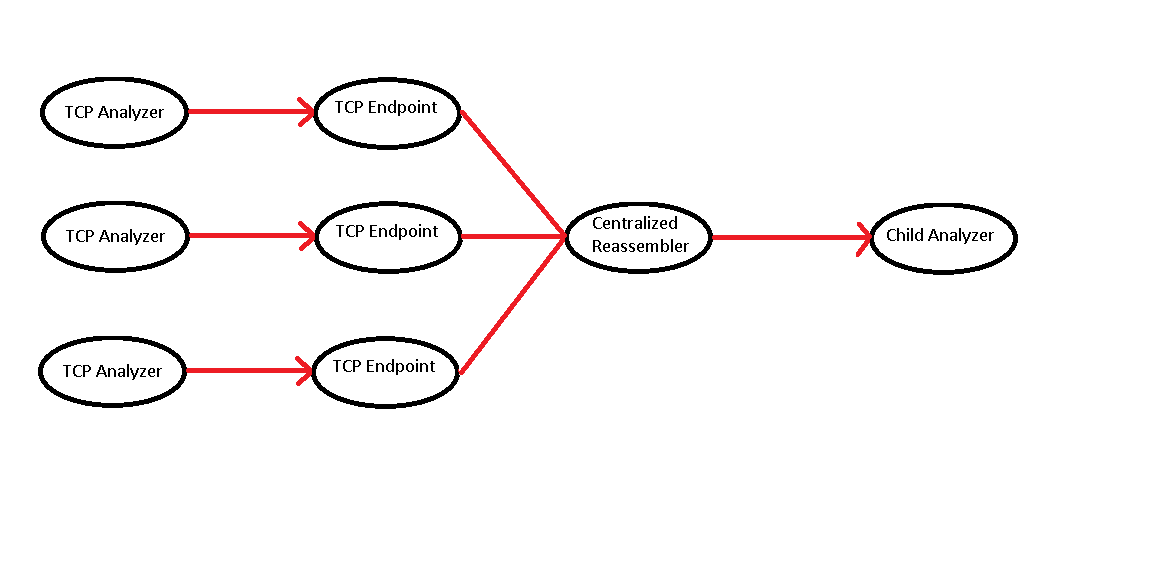
\includegraphics[width=\columnwidth]{Figures/manytoone.png}
\caption{Reassembling from Distinct Conns}
\label{pic:reassemblymany}
\end{figure}



\section{Interaction with the Implemented Changes} \label{sec:interf}

As we have seen, the original changes made to the Engine do not have any contribution to reassembly. However, we may now wonder whether or not the events created in the first implementation (and the scripts that use them) will still be usable. Unfortunately, while the events would still be raised, most of them contain the Conn ID as a means to retrieve the addresses and ports in the scripts. Since all the subflows now share the same Conn ID, it would be impossible to differentiate their addresses. This could be fixed by reading the address from the header in the Engine instead of relying on the ID when necessary.\\

However, the addresses are mainly used for the connection logging, which can now be done in a much simpler manner. Indeed, since the subflow matching is now performed in the Engine, it would be much simpler to add new events at that point, indicating when a flow has joined an existing connection. Simply put, while the "simpler" events can still be used, anything relating to connection establishment should be performed through new, higher-level events raised during the subflow matching. \\

Finally, it is worth noting that the option parsing of the reassembly cannot be turned off dynamically (depending on the scripts used) as is the case for the MPTCP events. Whether or not we are looking for any MPTCP activity, the Engine must still perform the MPTCP-related operations in order to ensure that no other analyzer suffers. This also leads to redundant computations in the case where we are processing MPTCP events. In order to cut back on the unnecessary processing, it would be advantageous to raise MPTCP events during the first parsing of the TCP options (in \texttt{Sessions.cc}). The issue of course is that the events would be raised at a somewhat unrelated stage of the packet analysis.